\section{Concept \& Design}
\label{sec: concept}
In this section we present the high-level architecture of the current ROMIO implementation as well as our proposed architecture. The two are shown in Figure~\ref{figure: romio-architecture} and~\ref{figure: new-romio-architecture} respectively. The ROMIO middleware is designed to be modular and easily extensible. Support for different parallel file systems is provided through additional software modules called drivers. The appropriate driver is selected at file open time through an interface called Abstract Device I/O (ADIO), following an approach similar to the Virtual File System layer of the Linux Kernel. 

\begin{figure}[!htb]
  \centering
  \begin{subfigure}[t]{0.38\textwidth}
  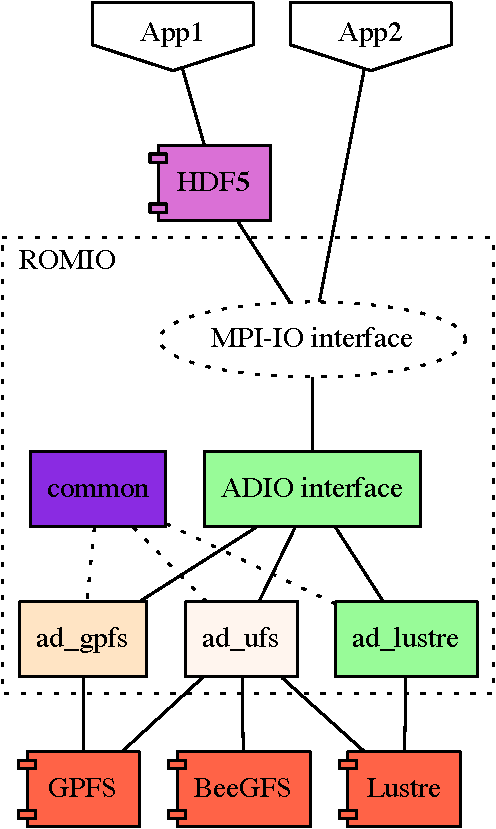
\includegraphics[width=\textwidth]{chapters/chapter3/figures/romio-architecture-src.pdf}
  \caption{ROMIO architecture}
  \label{figure: romio-architecture}
  \end{subfigure}
  \begin{subfigure}[t]{0.55\textwidth}
  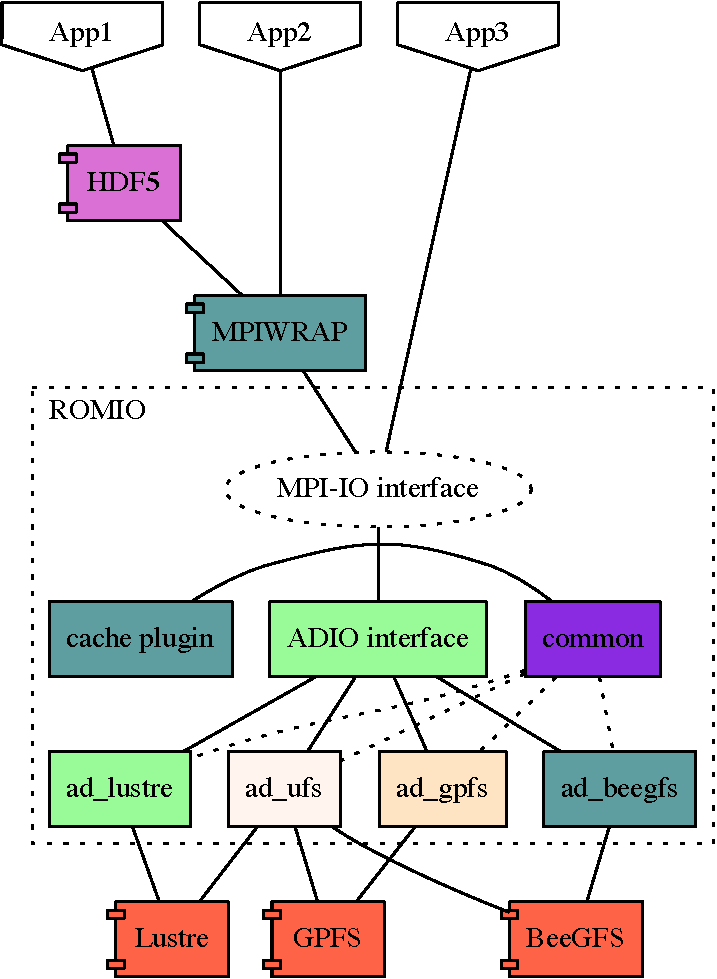
\includegraphics[width=\textwidth]{chapters/chapter3/figures/new-romio-architecture-src.pdf}
  \caption{Proposed ROMIO architecture}
  \label{figure: new-romio-architecture}
  \end{subfigure}
\end{figure}

In Figure~\ref{figure: romio-architecture} there are three different file system drivers: \textit{ad\_gpfs} for GPFS support, \textit{ad\_ufs} for Universal File System (UFS) support, and \textit{ad\_lustre} for Lustre support. These drivers share features implemented in the \textit{common} module. The common module contains the implementation for most of the I/O operations used by the UFS driver (ad\_ufs) and other drivers. File system drivers can implement their own I/O operations or use the ones made available by the common module. Lustre, for example, uses the common collective open operation (\codeword{ADIOI\_GEN\_Opencoll()}) but implements its own collective write operation (\codeword{ADIOI\_LUSTRE\_WriteStridedColl()}) described in Figure~\ref{figure: coll_io_impl}. Specific implementations are selected using a file operation table that has to be defined by every file system driver. Listing~\ref{list: lustre_table} shows the operation table for the ad\_lustre driver.

\begin{lstlisting}[language=C, caption=Operation Table for Lustre Driver, label={list: lustre_table}]
struct ADIOI_Fns_struct ADIO_LUSTRE_operations = {
    ADIOI_LUSTRE_Open, /* Open */
    ADIOI_GEN_OpenColl, /* OpenColl */
    ADIOI_LUSTRE_ReadContig, /* ReadContig */
    ADIOI_LUSTRE_WriteContig, /* WriteContig */
    ADIOI_GEN_ReadStridedColl, /* ReadStridedColl */
    ADIOI_LUSTRE_WriteStridedColl, /* WriteStridedColl */
    ADIOI_GEN_SeekIndividual, /* SeekIndividual */
    ADIOI_GEN_Fcntl, /* Fcntl */
    ADIOI_LUSTRE_SetInfo, /* SetInfo */
    ADIOI_GEN_ReadStrided, /* ReadStrided */
    ADIOI_LUSTRE_WriteStrided, /* WriteStrided */
    ADIOI_GEN_Close, /* Close */
#if defined(ROMIO_HAVE_WORKING_AIO) && !defined(CRAY_XT_LUSTRE)
    ADIOI_GEN_IreadContig, /* IreadContig */
    ADIOI_GEN_IwriteContig, /* IwriteContig */
#else
    ADIOI_FAKE_IreadContig, /* IreadContig */
    ADIOI_FAKE_IwriteContig, /* IwriteContig */
#endif
    ADIOI_GEN_IODone, /* ReadDone */
    ADIOI_GEN_IODone, /* WriteDone */
    ADIOI_GEN_IOComplete, /* ReadComplete */
    ADIOI_GEN_IOComplete, /* WriteComplete */
    ADIOI_GEN_IreadStrided, /* IreadStrided */
    ADIOI_GEN_IwriteStrided, /* IwriteStrided */
    ADIOI_GEN_Flush, /* Flush */
    ADIOI_GEN_Resize, /* Resize */
    ADIOI_GEN_Delete, /* Delete */
    ADIOI_GEN_Feature, /* Features */
    "LUSTRE:",
};
\end{lstlisting}

In Figure~\ref{figure: new-romio-architecture} we extend the presented ROMIO architecture with two additional modules: a dedicated driver supporting the BeeGFS file system (\textit{ad\_beegfs}) and a \textit{cache plugin} that links directly to the common module, thus providing NVM caching features to all the underlying file system drivers. We also developed an external library called \textit{MPIWRAP} that is used to allow transparent integration of the new caching functionalities into existing applications without any need of modifying them. 

In the rest of the chapter we describe in details the new MPI-IO hints supporting local NVM caching and the corresponding cache plugin module implementation.

\subsection{MPI-IO Hints Extensions}
%To the best of our knowledge there is currently very little or no work on how to use non-volatile memory devices in computing nodes of an HPC cluster as persistent cache layer to boost collective I/O performance in ROMIO. The use of these devices can greatly increase parallelism, reduce write response time variations among processes and consequently global synchronisation cost. Data cached in locally attached SSDs can be synchronised independently by every aggregator in the background while the application can progress doing useful work, effectively converting collective I/O to independent I/O when writing to the parallel file system.

To take advantage of attached non-volatile memories in computing nodes we introduced a new set of MPI-IO hints, reported in Table~\ref{table: hints_table}, and a corresponding set of modifications in the ROMIO implementation of the UFS driver supporting them.

\begin{table}[!htb]
\centering
\ra{1.5}
\caption{Proposed MPI-IO hints extensions.}
\newcolumntype{K}{>{\centering\arraybackslash} m{4cm}}
\newcolumntype{V}{>{\centering\arraybackslash} m{5cm}}
\begin{tabular}{KV}
\toprule
\bf \small Hint & \bf \small Value \\
\midrule
\small \codeword{e10\_cache} & \small \codeword{enable}, \codeword{disable}, \codeword{coherent}\\
\small \codeword{e10\_cache\_path} & \small cache directory pathname\\
\small \codeword{e10\_cache\_flush\_flag} & \small \codeword{flush\_immediate}, \codeword{flush\_onclose}, \codeword{flush\_none}\\
\small \codeword{e10\_cache\_discard\_flag} & \small \codeword{enable}, \codeword{disable}\\
\small \codeword{e10\_cache\_threads} & \small number of synchronisation thread in pool\\
\small \codeword{ind\_wr\_buffer\_size} & \small synchronisation buffer size [bytes]\\
\hline
\end{tabular}
\label{table: hints_table}
\end{table}

The new hints are used to control the data path in the storage system as well as to define a basic set of cache policies for synchronisation and space management. In particular, the \codeword{e10\_cache} hint is used to \codeword{enable} or \codeword{disable} the cache, directing applications' data to the local file system instead of the global file system. When the hint is set to \codeword{coherent} all the written data extents will be locked until cache synchronisation is completed. The \codeword{e10\_cache\_path} hint is used to control where, in the local file system tree, the cache file will reside. The \codeword{e10\_cache\_flush\_flag} hint is used to control the synchronisation policy of cached data to the global file. If the hint is set to \codeword{flush\_immediate} data will be immediately flushed to the global file. Alternatively, if the hint is set to \codeword{flush\_onclose} data will be flushed to the global file when it is closed. A \codeword{flush\_none} option is also provided to keep data local to the node and never flush it to the global file system. The \codeword{e10\_cache\_discard\_flag} hint is used to perform basic cache space management. In particular, if the hint is set to \codeword{enable} the cache file will be removed after the file is closed, otherwise (\codeword{disable}) it will be retained until the user manually removes it. The \codeword{e10\_cache\_threads} hint is used to communicate the implementation the number of threads that need to be created in the synchronisation thread pool when the file is opened (default is 1). Finally, the \codeword{ind\_wr\_buffer\_size} hint controls the size of the buffer used to synchronise cached data to the global file. This hint already existed in ROMIO but was only used during independent I/O to determine the write granularity. The hints in Table~\ref{table: hints_table} can be used in conjunction with the collective I/O hints described in section~\ref{subsec: hints}.

Besides the proposed cache policies, more complex ones are possible. For example, the cache synchronisation could take into account the level of congestion of the I/O servers. The cache replacement policy could also use a more complex strategy to evict cached files (or extents of data inside the file). Although these can be implemented in ROMIO, they introduce more sophisticated functionalities that go beyond the scope of this work.

\subsection{Cache Hints Integration in ROMIO}
\label{subsec: support}
As already mentioned, the introduced MPI-IO hints are supported by a corresponding set of modifications in the ROMIO implementation~\cite{E10-DEEPER} in the form of cache plugin. These modifications, following described, provide the functionalities necessary to handle the additional cache layer.

\subsubsection{Cache Synchronisation Request}
\label{subsubsec: cache-sync-req}
The \codeword{ADIOI\_Sync\_req\_t} object provides the infrastructure required to initialise/finalise, set/get attributes to/from synchronisation requests. Synchronisation requests are initialised by the main thread in the write function and submitted to a separate thread (synchronisation thread) which will satisfy them while the main thread can progress with useful work. Listing~\ref{list: sync-req} shows the object API.

\begin{lstlisting}[language=C, caption=Synchronisation Request API, label={list: sync-req}]
/* for ADIOI_Sync_req_{get,set}_key() */
enum {
  ADIOI_SYNC_TYPE = 0, /* sync req type        */
  ADIOI_SYNC_OFFSET,   /* sync req write off   */
  ADIOI_SYNC_DATATYPE, /* sync req datatype    */
  ADIOI_SYNC_COUNT,    /* sync req count       */
  ADIOI_SYNC_REQ,      /* sync req MPI_Request */
  ADIOI_SYNC_ERR_CODE, /* sync req error_code  */
  ADIOI_SYNC_FFLAGS,   /* sync req flush flag  */
  ADIOI_SYNC_ALL,      /* sync req all fields  */
  ADIOI_SYNC_REQ_ERR   /* sync req err code    */
};

struct ADIOI_Sync_req {
  int           type_;
  int           count_;
  int           error_code_;
  int           fflags_;
  ADIO_Offset   off_;
  MPI_Datatype  datatype_;
  ADIO_Request *req_;
};

/* Synchronisation Request Interfaces */
typedef struct ADIOI_Sync_req *ADIOI_Sync_req_t;

int ADIOI_Sync_req_init(ADIOI_Sync_req_t *, ...);
int ADIOI_Sync_req_init_from(ADIOI_Sync_req_t *, 
  ADIOI_Sync_req_t);
int ADIOI_Sync_req_fini(ADIOI_Sync_req_t *);
int ADIOI_Sync_req_get_key(ADIOI_Sync_req_t, ...);
int ADIOI_Sync_req_set_key(ADIOI_Sync_req_t, ...);
\end{lstlisting}

There are two types of synchronisation requests, \codeword{ADIOI\_THREAD\_SYNC} and \codeword{ADIOI\_THREAD\_SHUTDOWN}. The first is used to describe a written file extent that needs to be copied from the cache to the global file system, the second is used to shut down the synchronisation thread when the file is closed.

Every synchronisation request has a \codeword{MPI\_Request} handle used to start asynchronous copy of data from the cache to the global file system and to check upon request completion by the main thread using \codeword{MPI\_Wait()}.

\subsubsection{Cache Synchronisation Thread}
\label{subsubsec: cache-sync-thread}
The \codeword{ADIOI\_Sync\_thread\_t} object provides the infrastructure to initialise/finalise threads and to enqueue, flush and wait for synchronisation requests. A pool of synchronisation threads is created when the file is opened and destroyed when the file is closed. Listing~\ref{list: sync-thread} shows the object API.

\begin{lstlisting}[language=C, caption=Synchronisation Thread API, label={list: sync-thread}]
enum {
  ADIOI_THREAD_SYNC = 0,
  ADIOI_THREAD_SHUTDOWN
};

struct ADIOI_Sync_thread {
  ADIO_File            fd_;
  pthread_t            tid_;
  pthread_attr_t       attr_;
  ADIOI_Atomic_queue_t sub_;
  ADIOI_Atomic_queue_t pen_;
  ADIOI_Atomic_queue_t wait_;
};

typedef struct ADIOI_Sync_thread *ADIOI_Sync_thread_t;

int  ADIOI_Sync_thread_init(ADIOI_Sync_thread_t *, ...);
int  ADIOI_Sync_thread_fini(ADIOI_Sync_thread_t *);
void ADIOI_Sync_thread_enqueue(ADIOI_Sync_thread_t, 
  ADIOI_Sync_req_t);
void ADIOI_Sync_thread_flush(ADIOI_Sync_thread_t);
void ADIOI_Sync_thread_wait(ADIOI_Sync_thread_t);
\end{lstlisting}

The synchronisation thread object has three queues, a pending queue (\textit{pen\_}), a submission queue (\textit{sub\_}) and a wait queue (\textit{wait\_}). New synchronisation requests are first added to the pending queue using the \codeword{ADIOI\_Sync\_thread\_enqueue()} function. Pending requests are not satisfied until they are moved to the submission queue using the \codeword{ADIOI\_Sync\_thread\_flush()} function. This function also pushes a copy of the request pointer to the wait queue, which is later used by the \codeword{ADIOI\_Sync\_thread\_wait()} function to wait for submitted requests to complete.

\subsubsection{Synchronisation Thread Pool Initialisation}
\label{subsubsec: thread-pool-init}
The thread pool is initialised in \codeword{ADIOI\_GEN\_Opencoll()}. This function is invoked by \codeword{MPI\_File\_open()} every time a new file is opened. Listing~\ref{list: open-coll} shows the code responsible for opening the cache file in the local file system and to start the synchronisation threads.

\begin{lstlisting}[language=C, caption=Synchronisation Thread Initialisation, label={list: open-coll}]
void ADIOI_GEN_Opencoll(...) {
  ...
  /* check cache mode */
  if (fd->hints->e10_cache == ADIOI_HINT_ENABLE) {
    /* get MPI_File handle for cache and init it */
    MPI_File mpi_fh = MPIO_File_create(sizeof(
      struct ADIOI_FileD));
    fd->cache_fd = MPIO_File_resolve(mpi_fh);
    fd->cache_fd->filename = ADIOI_GetCacheFilePath(
      fd->filename, fd->hints->e10_cache_path);
    fd->cache_fd->file_system = fd->file_system;
    fd->cache_fd->fns = fd->fns;
    fd->cache_fd->cache_fd = ADIO_FILE_NULL;

    ...

    /* every process tries opening the cache file */
    (*(fd->fns->ADIOI_xxx_Open))(fd->cache_fd,
      error_code);

    ...

    /* init synchronisation thread pool */
    if (*error_code == MPI_SUCCESS && 
        fd->hints->e10_cache_flush_flag != 
          ADIOI_HINT_FLUSHNONE) {
      if (fd->hints->cb_write == ADIOI_HINT_ENABLE)
        if (fd->is_agg)
          *error_code = 
            ADIOI_Sync_thread_pool_init(fd, NULL);
        else
          *error_code = MPI_SUCCESS;
      else
        *error_code = ADIOI_Sync_thread_pool_init(
          fd, NULL);
    }

    /* check every process has returned success */
    MPI_Allreduce(error_code, &max_error_code, 1, 
      MPI_INT, MPI_MAX, fd->comm);

    if (max_error_code != MPI_SUCCESS) {
      if (*error_code == MPI_SUCCESS ||
          *error_code == ADIOI_ERR_THREAD_CREATE) {
        (*(fd->fns->ADIOI_xxx_Close))(fd->cache_fd,
          error_code);
        if ((fd->cache_fd->access_mode & ADIO_CREATE) &&
            (fd->cache_fd->access_mode & 
              ADIO_DELETE_ON_CLOSE)) {
          ADIO_Delete(fd->cache_fd->filename, error_code);
        }
        /* fini synchronisation thread pool */
        if (fd->hints->e10_cache_flush_flag != 
            ADIOI_HINT_FLUSHNONE && fd->thread_pool) {
          ADIOI_Sync_thread_pool_fini(fd);
        }
      }

      /* Revert to standard file access: no cache */
      ADIOI_Info_set(fd->info, "e10_cache", "disable");
      fd->hints->e10_cache = ADIOI_HINT_DISABLE;
    } else {
      fd->cache_fd->is_open = 1;
    }
  }
  ...
}
\end{lstlisting}

In order for the implementation to exploit local NVM caching both local file creation and thread initialisation must succeed. The MPI file handle for the cache file is stored in \textit{cache\_fd} inside the file handle of the global file. When collective I/O is enabled only the aggregators will initialise the synchronisation thread pool. In any other case every process will do independent I/O and will thus initialise its own pool.

\subsubsection{Synchronisation Request Submission}
\label{subsubsec: sync-req-sub}
\codeword{ADIOI\_GEN\_WriteContig()} is the function responsible for writing data to the file. This function is used by both collective and independent I/O. We have extended the write function to support creation and submission of new synchronisation requests to the thread pool. Listing~\ref{list: req-sub} shows the corresponding implementation.

\begin{lstlisting}[language=C, caption=Synchronisation Request Submission, label={list: req-sub}]
void ADIOI_GEN_WriteContig(...) {
  ...

  /* if using the cache select the cache file handle */
  if (fd->cache_fd && fd->cache_fd->is_open) {
    fh = fd->cache_fd;

    /* if cache is coherent lock global file extent */ 
    if (fd->hints->e10_cache_coherent == ADIOI_HINT_ENABLE)
      ADIOI_WRITE_LOCK(fd, offset, SEEK_SET, len);
  }

  /* write to the cache file handle */

  /* init and submit sync request */
  if (fd->cache_fd && fd->cache_fd->is_open && 
      fd->hints->e10_cache_flush_flag != 
        ADIOI_HINT_FLUSHNONE) {
    ADIOI_Sync_req_t sub;
    int threads, curr_thread, idx;
    ADIO_Request *r = (ADIO_Request *)ADIOI_Malloc(
      sizeof(ADIO_Request));

    *r = MPI_REQUEST_NULL;
    threads = fd->hints->e10_cache_threads;
    curr_thread = fd->thread_curr;
    idx = curr_thread % threads;

    /* init sync req */
    ADIOI_Sync_req_init(&sub, ADIOI_THREAD_SYNC, offset, 
      datatype, count, r, 0);

    /* enqueue sync request to thread and flush */
    ADIOI_Sync_thread_enqueue(fd->thread_pool[idx], sub);
    if (fd->hints->e10_cache_flush_flag == 
        ADIOI_HINT_FLUSHIMMEDIATE)
      ADIOI_Sync_thread_flush(fd->thread_pool[idx]);

    /* select next thread in the pool */
    fd->thread_curr = (curr_thread + 1) % threads;
  }
}
\end{lstlisting}

For each write a new synchronisation request is initialised using the same set of I/O parameters (i.e. offset, datatype, count, etc) as the original write operation. The request is then enqueued to the appropriate thread in the pool using \codeword{ADIOI\_Sync\_thread\_enqueue()}. If the \codeword{e10\_cache\_flush\_flag} is set to \codeword{flush\_immediate} the request is immediately scheduled to be served by invoking \codeword{ADIOI\_Sync\_thread\_flush()}, otherwise it will be flushed when the file is closed.

\subsubsection{Cache Flushing}
\label{subsubsec: cache-flush}
\codeword{ADIOI\_GEN\_Flush()} is the function responsible for flushing the page cache. This function is used by \codeword{MPI\_File\_sync()}. We have extended the file flush function to support flushing and waiting of outstanding synchronisation requests. Listing~\ref{list: req-flush} shows the corresponding implementation.

\begin{lstlisting}[language=C, caption=Cache Flushing, label={list: req-flush}]
void ADIOI_GEN_Flush(...) {

  ...

  if (fd->cache_fd == NULL || fd->thread_pool == NULL ||
      (fd->cache_fd && !fd->cache_fd->is_open) ||
      (fd->cache_fd && fd->cache_fd->is_open &&
      fd->hints->e10_cache_flush_flag == ADIOI_HINT_FLUSHNONE))
    goto fn_flush;

  threads = fd->hints->e10_cache_threads;

  /* Flush all the requests in each thread */
  for (idx = 0; idx < threads; idx++) {
    ADIOI_Sync_thread_flush(fd->thread_pool[idx]);
  }

  /* Wait for submitted requests to complete */
  for (idx = 0; idx < threads; idx++) {
    ADIOI_Sync_thread_wait(fd->thread_pool[idx]);
  }
  return;

fn_flush:
  /* fsync global file handle */
}
\end{lstlisting}

When invoked, the flush routine will trigger cache synchronisation for every thread in the pool by invoking \codeword{ADIOI\_Sync\_thread\_flush()}. As previously described this will move all the requests in the pending queue to the submission queue to be served. If the pending queue is empty, the thread flush routine will return immediately. Once all the threads in the pool have been flushed, the routine waits on each of them to complete by invoking \codeword{ADIOI\_Sync\_thread\_wait()} and finally returns.

\subsubsection{Synchronisation Thread Pool Finalisation}
\label{subsubsec: thread-pool-fini}
\codeword{ADIO\_Close()} is the function responsible for closing a file. This function is used by \codeword{MPI\_File\_close()}. We have extended the close function to support closing of cache file and finalisation of the synchronisation thread pool. Listing~\ref{list: thread-fini} shows the corresponding implementation.

\begin{lstlisting}[language=C, caption=Synchronisation Thread Pool Finalisation, label={list: thread-fini}]
void ADIO_Close(...) {

  ...

  if (fd->cache_fd) {
    if (fd->cache_fd->is_open) {
      /* First check if there is any outstanding sync */
      (*(fd->fns->ADIOI_xxx_Flush))(fd, error_code);

      /* Afterwards we can close the cache file */
      (*(fd->fns->ADIOI_xxx_Close))(fd->cache_fd, 
        error_code);

      /* Finilise thread pool */
      ADIOI_Sync_thread_pool_fini(fd);
    }

    /* Only the process that created the file deletes it */
    if ((fd->cache_fd->access_mode & ADIO_CREATE) &&
        (fd->cache_fd->access_mode & ADIO_DELETE_ON_CLOSE))
      ADIO_Delete(fd->cache_fd->filename, &err);

    /* Free cache_fd */
    ADIOI_Free(fd->cache_fd->filename);
    MPIO_File_free(&(fd->cache_fd));
    fd->cache_fd = ADIO_FILE_NULL;
  }

  ...

}
\end{lstlisting}

When invoked, the close routine will trigger the flushing of the cache (\codeword{(*(fd->fns->ADIOI\_xxx\_Flush))()}), close the cache file (\codeword{(*(fd->fns->ADIOI\_xxx\_Close))()}) and finalise the thread pool (\codeword{ADIOI\_Sync\_thread\_pool\_fini()}).

\begin{figure}[!htb]
  \centering
  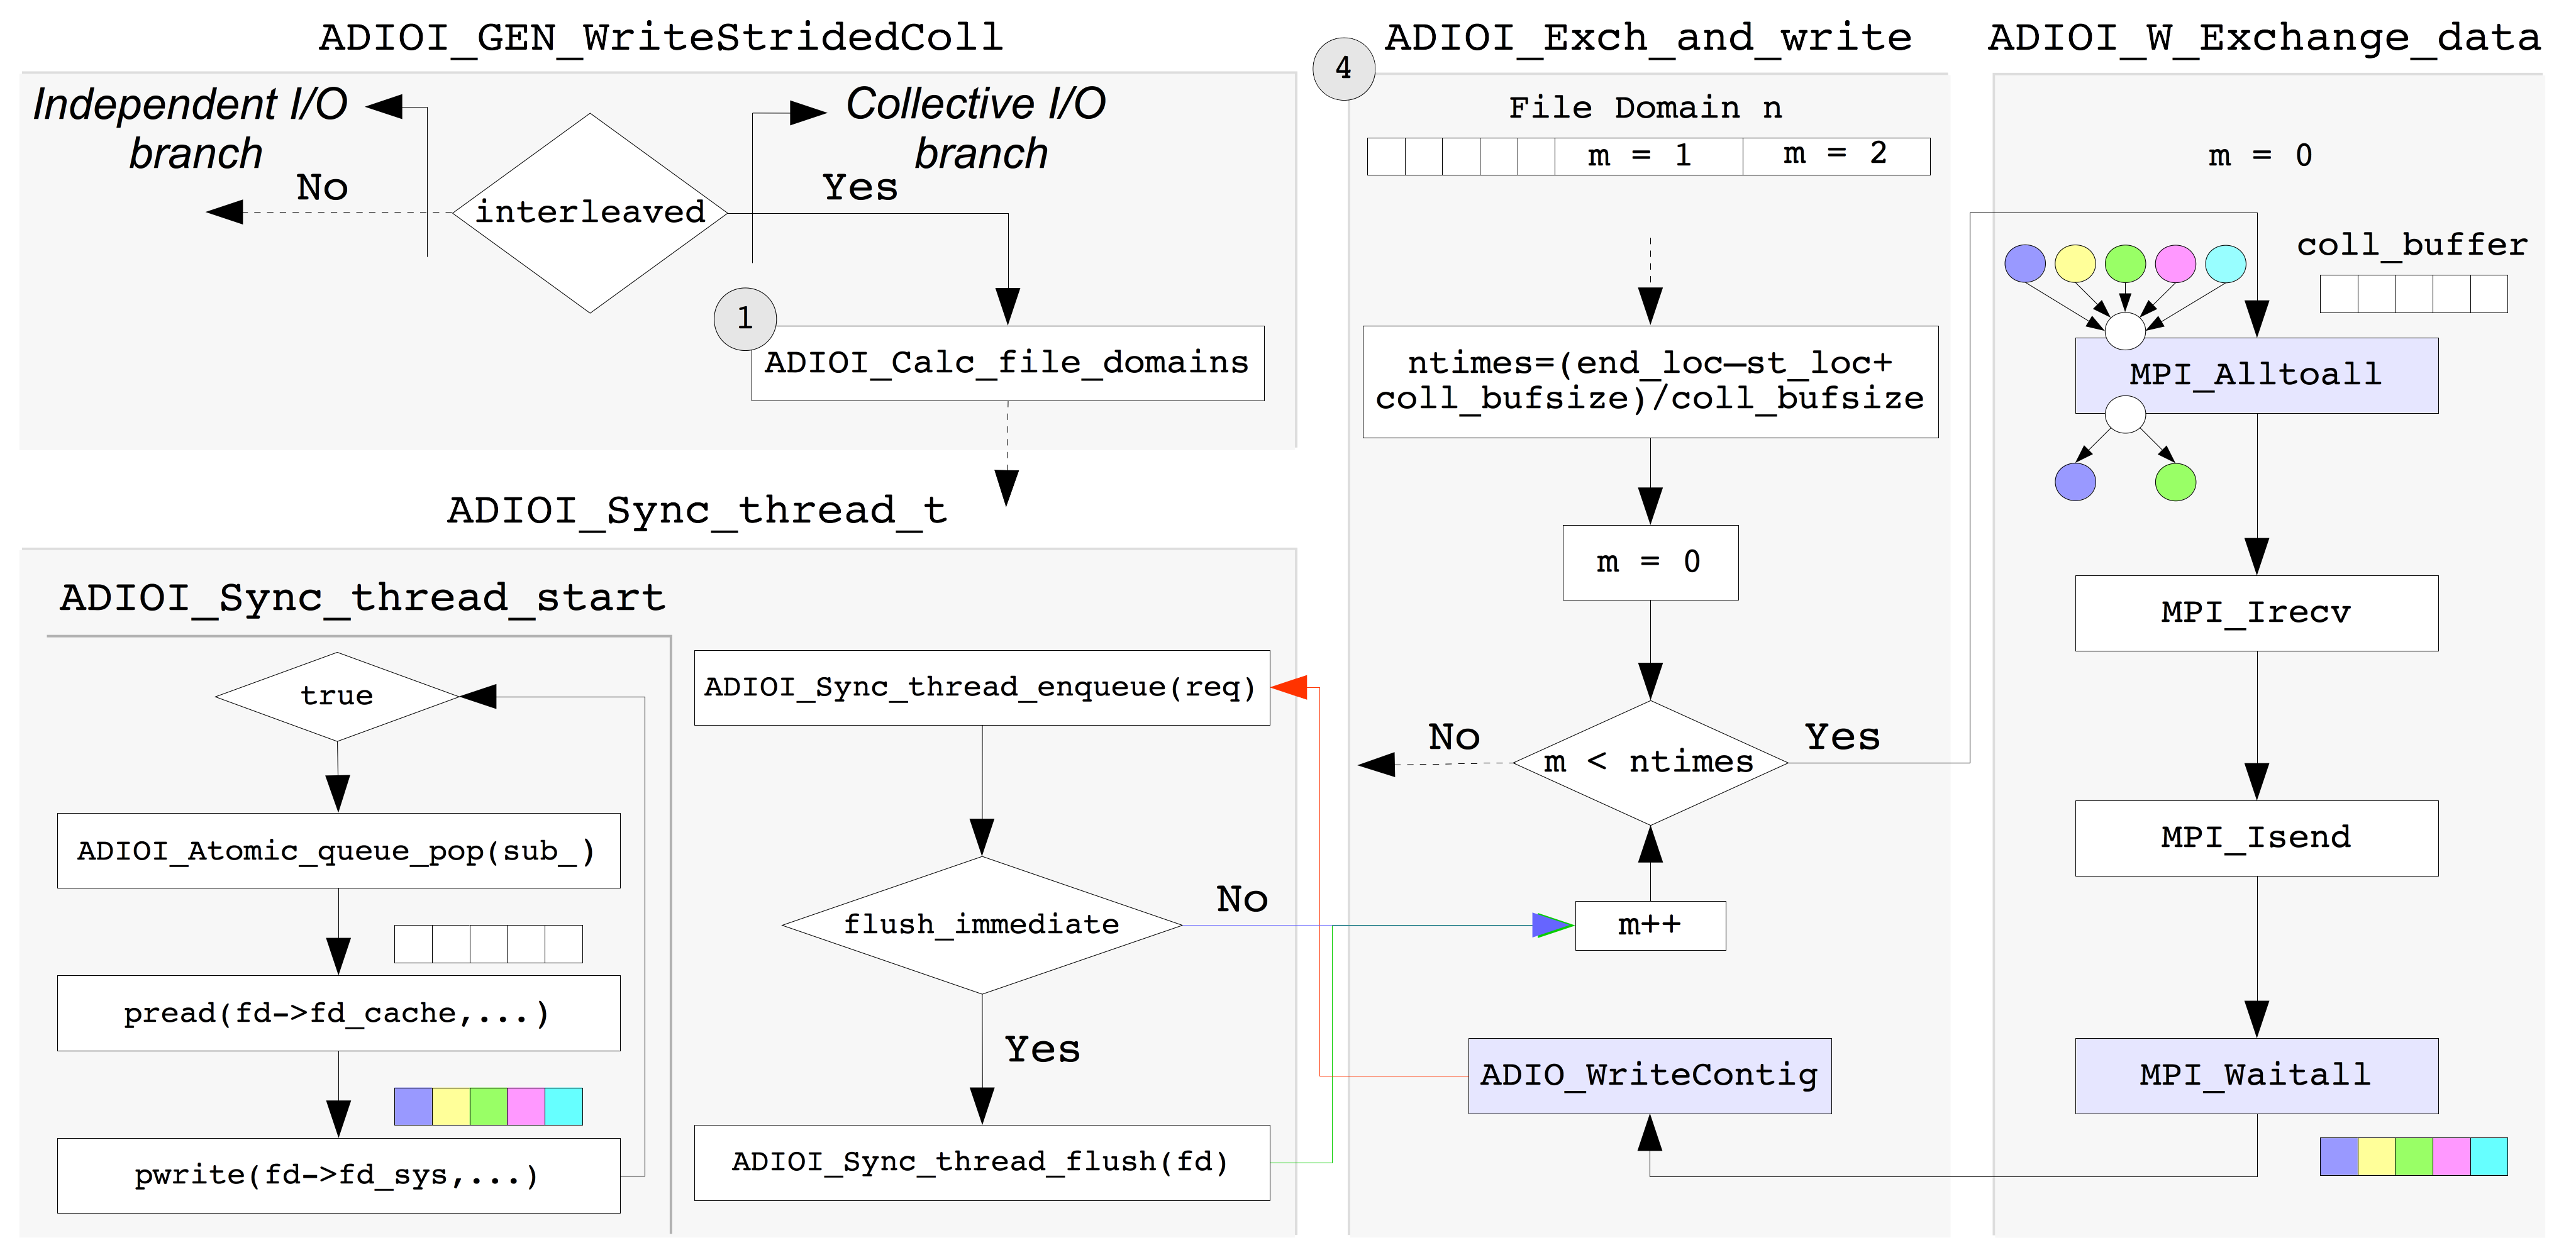
\includegraphics[width=\textwidth]{chapters/chapter3/figures/ext2ph+e10}
  \caption{New Collective I/O flow diagram.}
  \label{figure: new_coll_io_impl}
\end{figure}

Figure~\ref{figure: new_coll_io_impl} graphically shows the modified flow diagram for the new collective I/O implementation just described. Compared to Figure~\ref{figure: coll_io_impl}, there is now an additional component representing the synchronisation thread. When data is written to the cache file, a synchronisation request for the written data is initialised and submitted to the \codeword{ADIOI\_Sync\_thread\_t} object. The object's pthread continuously search in the submission queue (\textit{sub\_}) for new synchronisation requests to satisfy.

\subsection{BeeGFS Cache Integration in ROMIO}
The BeeGFS file system provides its own caching infrastructure, which includes a set of APIs to control the caching functionalities and a deamon process, running on the host machine, that takes care of moving data between the cache and the global file system. For this reason, some of the cache plugin features presented before for the universal file system module are redundant. In particular, we do not any longer need to manually open a cache file in the host and start a pool of synchronisation threads. When using the BeeGFS cache API the file system will take care of all these aspects for us. Nevertheless, we can still recycle some part of the cache plugin as described below.

\subsubsection{Cache Opening}
The BeeGFS collective open function is implemented in \codeword{ADIOI\_BEEGFS\_OpenColl()}. This will be automatically invoked when \codeword{MPI\_File\_open()} is called by the application. The implementation for the collective open is similar to the universal file system implementation and is reported in Listing~\ref{list: beegfs_opencoll}.

\begin{lstlisting}[language=C, caption=BeeGFS Collective Open Implementation, label={list: beegfs_opencoll}]
void ADIOI_BEEGFS_OpenColl(...) {

  ...

  /* workout parent directory for file */
  dir = ADIOI_Dirname(fd->filename);

fn_open:
  if (access_mode & ADIO_CREATE) {
    if (rank == fd->hints->ranklist[0]) {
      /* remove delete on close flag if set */
      if (access & ADIO_DELETE_ON_CLOSE)
        fd->access_mode = access_mode ^ 
                          ADIO_DELETE_ON_CLOSE;
      else
        fd->access_mode = access_mode;
      
      /* prefetch the parent dir into the cache */
      if (fd->hints->e10_cache == ADIOI_HINT_ENABLE) {
        ret = deeper_cache_prefetch(dir, 
                DEEPER_PREFETCH_SUBDIR | 
                DEEPER_PREFETCH_WAIT);

        /* enforce synchronous flush 
         * when closing the file */
        fd->cache_oflags = DEEPER_OPEN_FLUSHONCLOSE | 
                           DEEPER_OPEN_FLUSHWAIT;
      } else {
        ret = DEEPER_RETVAL_SUCCESS;
      }

      ...

      /* only the rank 0 process creates the file 
       * invoking deeper_cache_open() */
      if (ret == DEEPER_RETVAL_SUCCESS || 
           (ret == DEEPER_RETVAL_ERROR && errno == EEXIST)) 
      {
        (*(fd->fns->ADIOI_xxx_Open))(fd, error_code);
      }

      /* close the cache file forcing BeeGFS to flush it */
      if (*error_code == MPI_SUCCESS)
        (*(fd->fns->ADIOI_xxx_Close))(fd, error_code);

      MPI_Bcast(error_code, 1, MPI_INT, 
                fd->hints->ranklist[0], fd->comm);

      /* restore the delete on close flag if it was set */
      fd->access_mode = access_mode;
    } else {
      MPI_Bcast(error_code, 1, MPI_INT, 
                fd->hints->ranklist[0], fd->comm);
    }

    /* check cache errors and if any revert 
     * to standard I/O */
  }

  /* now every process opens the file */

  if (fd->hints->e10_cache == ADIOI_HINT_ENABLE) {
    deeper_cache_prefetch(dir, DEEPER_PREFETCH_SUBDIR |
                               DEEPER_PREFETCH_WAIT);

    /* default open flags */
    fd->cache_oflags = DEEPER_OPEN_FLUSHONCLOSE | 
                       DEEPER_OPEN_FLUSHWAIT;

    if (fd->hints->e10_cache_discard_flag == 
        ADIOI_HINT_ENABLE)
      fd->cache_oflags |= DEEPER_OPEN_DISCARD;

  }

  (*(fd->fns->ADIOI_xxx_Open))(fd, error_code);

  ...

}
\end{lstlisting}

Similarly to before, the rank 0 process needs to setup the cache by prefetching the file parent directory into the cache, through \codeword{deeper\_cache\_prefetch()}. Afterwards, rank 0 opens the file inside the prefetched directory by invoking the local open (\codeword{ADIOI\_BEEGFS\_Open()}). The local open performs the real open operation using \codeword{deeper\_cache\_open()} instead of \codeword{open()}. If the open succeeds the cache file is closed, thus forcing BeeGFS to mirror it in the global file system. At this point all the other processes can prefetch the parent directory and the file created by rank 0 inside it.

By default the cache open flags for the file, \codeword{fd->cache\_oflags}, are always set to DEEPER\_FLUSHONCLOSE and DEEPER\_FLUSHWAIT; this means that if there is any non-synchronised data in the cache, the close operation will force this data to be flushed to the global file system and will not return until all the data has been copied.

\subsection{Cache Consistency Semantics}
\label{subsec: consistency}
As far as write consistency is concerned, the MPI-IO interface does not make any assumption regarding the underlying storage system or its semantics. ROMIO specifically supports file systems that are both POSIX compliant, like Lustre, and non-POSIX compliant, like NFS or PVFS. In MPI-IO, written data becomes globally visible only after either \codeword{MPI\_File\_sync()} or \codeword{MPI\_File\_close()} are invoked on the MPI file handle and by default there is no write atomicity. The motivation is that data can be cached at some level locally in the compute nodes. The ROMIO implementation can overcome the risk of data inconsistency, e.g. related to false sharing of file system blocks, using persistent file realms~\cite{ColomaCWWRP04}, and can even enforce atomicity using \codeword{MPI\_File\_set\_atomicity()}.

In our implementation we comply to the MPI-IO semantics just described. This means that data written to the local file system cache using the newly introduced MPI-IO hints will be globally visible to the rest of the nodes only under the following circumstances:
\begin{itemize}
\item The \codeword{e10\_cache\_flush\_flag} has been set to \codeword{flush\_immediate} by the user and synchronisation, started automatically by the implementation right after the write operation, has completed;
\item The \codeword{e10\_cache\_flush\_flag} has been set to \codeword{flush\_onclose} by the user and the invoked \codeword{MPI\_File\_close()} has returned;
\item The \codeword{MPI\_File\_sync()} function has been invoked by the user and it has returned.
\end{itemize}

Consistency for reading data from the cache is not clearly defined by the ext2ph algorithm. In general, data written to the local file system cache can be read back from the user without accessing the global file system. Nevertheless, the algorithm calculates the location of a data block based on the number of aggregators, their logical position within the set of aggregators, and the size of the complete data set. This means that a collective read that matches the previous write could safely read the data from the aggregators' cache without incurring any problem. In spite of that, in general reading from the cache requires additional metadata describing the file layout across the caches. For this reason, we currently do not support reads from the local file system cache.

Furthermore, whenever required, we can enforce cache coherency ensuring that read operations cannot access data that is currently in transit, i.e., not or only partially moved from the cache to the global file. This can be done by locking the file domain extent being cached until all the data has been made persistent in the global file. For this purpose ROMIO provides a set of internal locking macros, namely \codeword{ADIOI\_WRITE\_LOCK}, \codeword{ADIOI\_READ\_LOCK} and \codeword{ADIOI\_UNLOCK} that we used in our implementation. The lock of cached data can be selected by setting the \codeword{e10\_cache} hint in Table~\ref{table: hints_table} to \codeword{coherent}. This will \codeword{enable} the cache and set locks appropriately, assuming underlying file system support.

\subsection{Changes to the Application's Workflow}
\label{subsec: new-workflow}
Simplifying, most HPC applications can be divided into multiple phases of computation, in which data is produced, and I/O, in which data is written to persistent storage for post-processing purposes as well as defensive checkpoint-restart. Focusing on the I/O phase and considering the case of applications writing to a shared file, the I/O phase can be divided into the following steps:
\begin{enumerate}
        \item The file is opened using \codeword{MPI\_File\_open()}: at this point the info object containing the user defined MPI-IO hints is passed to the underlying ROMIO layers.
        \item Data is written to the file using \codeword{MPI\_File\_write\_all()}: these functions invoke the underlying \codeword{ADIOI\_GEN\_WriteStridedColl()} previously described in Figure~\ref{figure: coll_io_impl}.
        \item The file is closed using \codeword{MPI\_File\_close()}: after the file is closed data must be visible to every process in the cluster. 
\end{enumerate}

To take advantage of the proposed MPI-IO hint extensions, the application's workflow has to be modified. Figure~\ref{figure: workflow3} shows the classical application's workflow (cache disabled) as well as the modified version using the new hints (cache enabled). The difference is that, in order to take advantage of the proposed hints and hide the cache synchronisation to the computation phase, the \codeword{MPI\_File\_close()} for the I/O phase `k' has been moved at the beginning of the I/O phase `k+1', just before the new file is opened.
\begin{figure}[!htb]
  \centering
  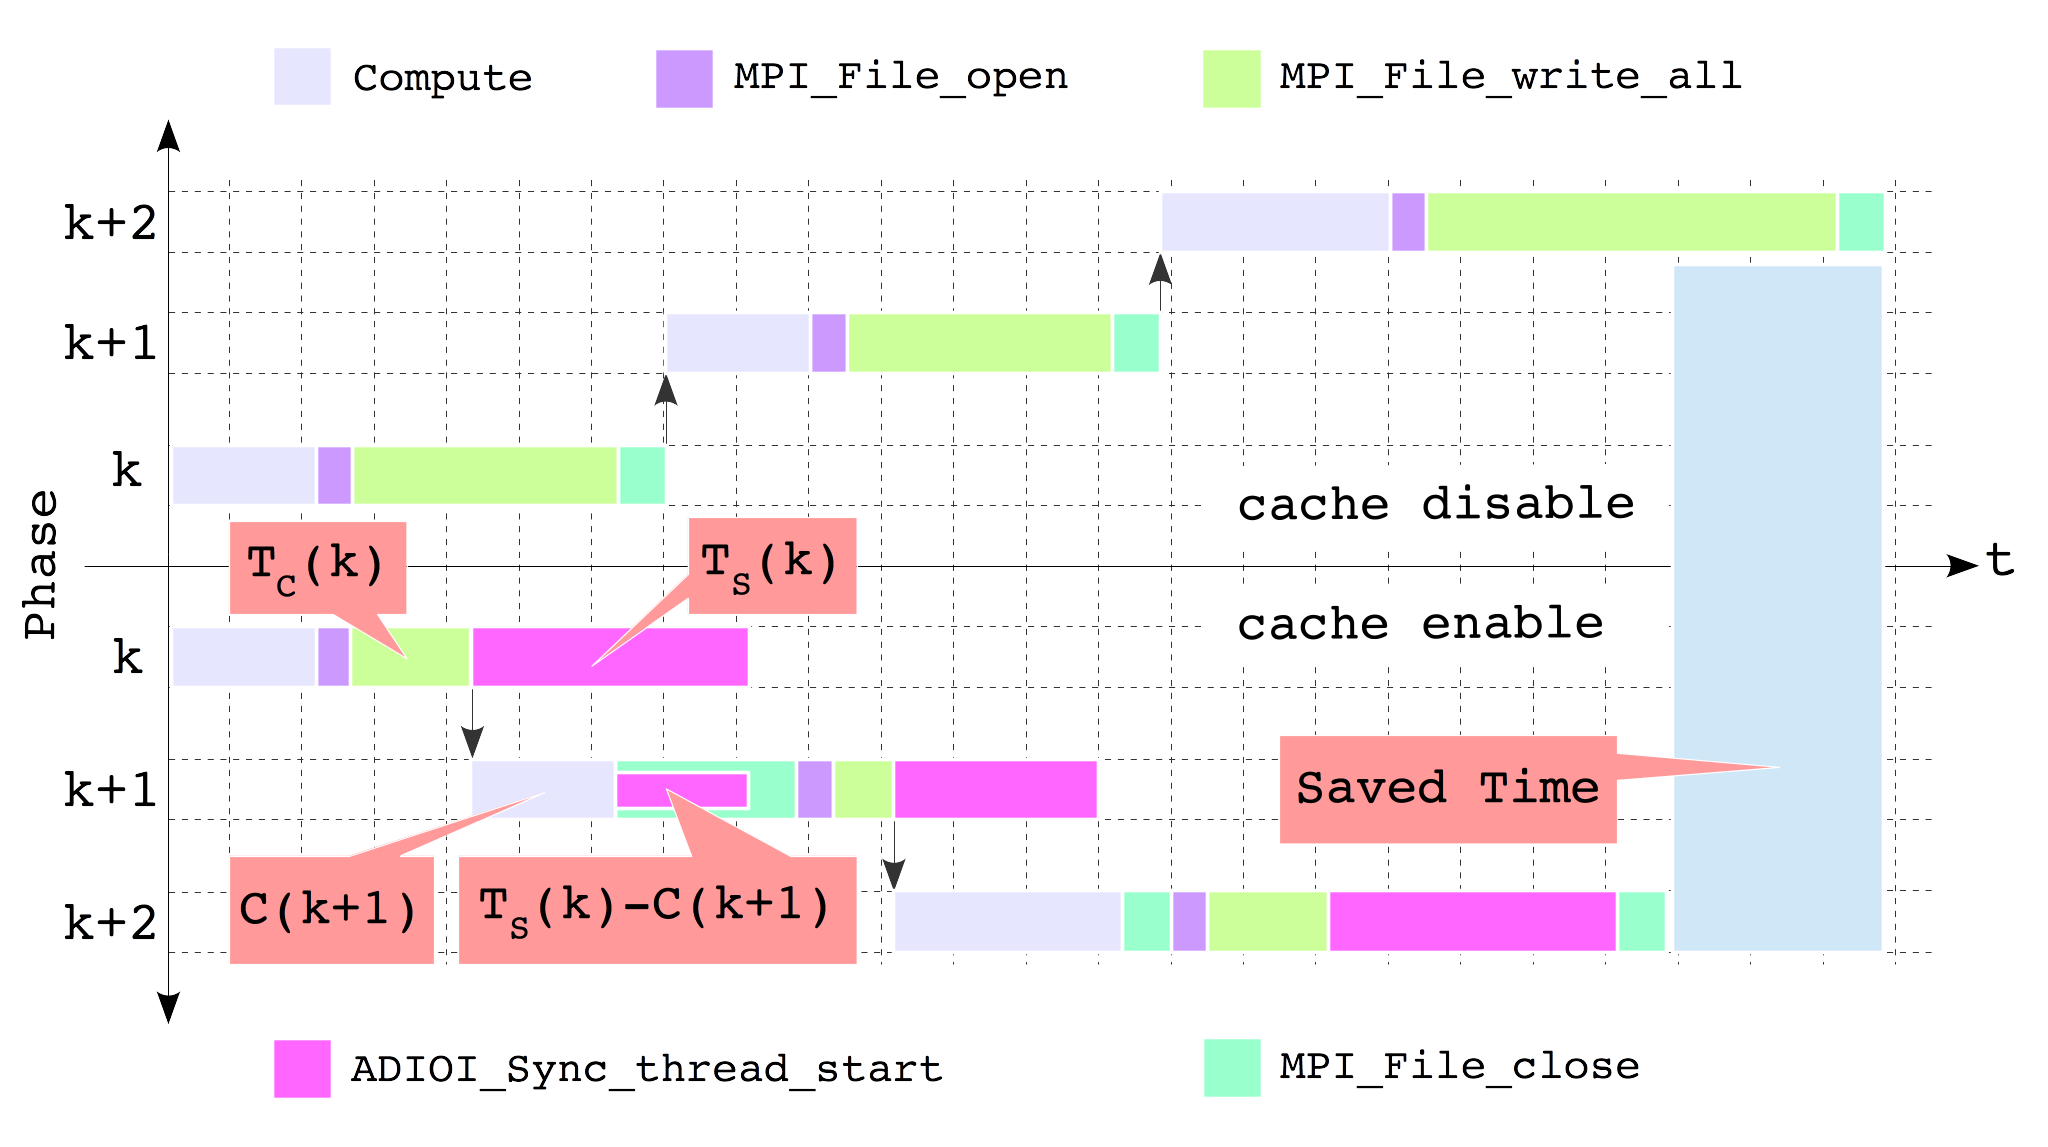
\includegraphics[width=0.9\textwidth]{chapters/chapter3/figures/workflow}
  \caption{Standard and modified workflows. When cache is disabled compute phase `k+1' starts after file `k' has been closed. When the cache is enabled compute `k+1' can start immediately after data has been written. At the same time, background synchronisation of cached data starts. File `k' is closed before the file `k+1' is opened, forcing the implementation to wait for cache synchronisation to complete.}
  \label{figure: workflow3}
\end{figure}

\subsubsection{MPIWRAP Library}
\label{subsubsec: mpiwrap}
Since the workflow modification just presented might not be feasible for legacy applications, we developed a MPI-IO wrapper library (called MPIWRAP), written in C++, that can reproduce this change behind the scenes. The library can be linked to the application or preloaded with \codeword{LD\_PRELOAD} and has been used for all the experiments contained in this thesis. MPI-IO hints are defined in a configuration file and passed by the library to \codeword{MPI\_File\_open()}. We can define multiple hints targeting different files or groups of files. The library overloads \codeword{MPI\_\{Init,Finalize\}()} and \codeword{MPI\_File\_\{open,close\}()} using the PMPI profiling interface. The workflow modification can be triggered for a specific set of files (identified by the same base name) in the configuration file. Whenever one of such files is closed, our \codeword{MPI\_File\_close()} implementation will return success. Nevertheless, the file will not be really closed. Instead, its handle will be kept internally for future references. When the next shared file with the same base name is opened, our \codeword{MPI\_File\_open()} implementation will search for outstanding opened file handles and will invoke \codeword{PMPI\_File\_close()} on them before opening the new file, thus triggering the cache synchronisation completion check for each of them.

\subsection{I/O Bandwidth}
\label{subsec: bw-impr}
According to the new I/O workflow, described in this section, we have that being $S(k)$ the amount of data written during phase `k', $T_c(k)$ the time needed to write $S(k)$ collectively to the cache using \codeword{MPI\_File\_write\_all()}, $T_s(k)$ the time needed to synchronise the cached data in every aggregator to the global file system (through \codeword{ADIOI\_Sync\_thread\_start()}), and $C(k+1)$ the computation time of phase `k+1', the resulting I/O bandwidth for `k' is expressed by Equation~\ref{formula: bw}:

\begin{equation}\label{formula: bw}
        bw(k) = \frac{S(k)}{T_c(k) + max(0,\ T_s(k) - C(k+1))}
\end{equation}
Therefore, the total average bandwidth perceived by the application is:
\begin{equation}\label{formula: abw}
        BW = \frac{\sum_{k=0}^{N-1} S(k)}{\sum_{k=0}^{N-1} T_c(k) + max(0,\ T_s(k) - C(k+1))}
\end{equation}

From Equation~\ref{formula: bw} (in which we have considered the open time neglectable) it is clear that the maximum performance can be obtained when $C(k+1) \geq T_s(k)$, that is, when we can completely hide cache synchronisation by the computation phase. On the other hand when $C(k+1) < T_s(k)$ we might have a minima in the bandwidth since \codeword{MPI\_File\_close()} needs to wait for cache synchronisation completion (Figure~\ref{figure: workflow3}). 
